\documentclass[10pt,twocolumn]{article}
\usepackage[letterpaper,margin=0.68in,columnsep=0.25in]{geometry}
\usepackage[T1]{fontenc}
\usepackage{lmodern}
\usepackage{microtype}
\usepackage{graphicx}
\usepackage{booktabs}
\usepackage{amsmath}
\usepackage[numbers,sort&compress]{natbib}
\usepackage[hidelinks]{hyperref}
\hypersetup{
  pdftitle={Within-traversal position-decoding deviations covary between hippocampal CA1 and retrosplenial cortex},
  pdfauthor={Javier Emilio Bazan Sanchez}
}
\usepackage{xcolor}
\usepackage{titlesec}
\usepackage{caption}
\captionsetup{font=small,labelfont=bf}
\titleformat{\section}{\large\bfseries}{\thesection}{0.55em}{}
\titleformat{\subsection}{\normalsize\bfseries}{\thesubsection}{0.5em}{}
\setlength{\parindent}{1em}
\setlength{\parskip}{0pt}

\title{Within-traversal position-decoding deviations covary between hippocampal CA1 and retrosplenial cortex}
\author{Javier Emilio Bazan Sanchez\\
\small Facultad de Ciencias, Universidad Nacional Autonoma de Mexico\\
\small \texttt{bazan@ciencias.unam.mx}}
\date{}

\begin{document}
\maketitle

\begin{abstract}
Hippocampal and cortical populations can encode the same spatial variable while using different neural codes. Whether their moment-to-moment spatial estimates fluctuate together is known for CA1--visual and CA1--prefrontal networks, but has not been tested for the hippocampal--retrosplenial axis. We analyzed simultaneous CA3, CA1, and deep-layer retrosplenial cortex (RSC) recordings from freely moving mice. Independent conditional-multinomial decoders were trained in odd/even traversal folds. We removed measured position, nonlinear speed, and trial-order effects at 250-ms resolution, averaged residuals within traversal-by-position cells, and compared same-traversal CA1--RSC correlations with a complete-group cyclic trial-rotation reference. In 12 exploratory sessions, the equal-mouse excess Fisher correlation was 0.2042 ($p=0.0001$; four of four mice positive). A frozen one-shot analysis of three reserved fixed-condition sessions confirmed the effect (excess Fisher $z=0.1465$, $p=0.0001$; three of three mice positive). Confirmation survived adjustment for CA1, RSC, and CA3 population spike totals (0.1331), adjustment for the independently decoded CA3 deviation (0.1392), and reconstruction from the opposite tracking-frame parity (0.1524; all $p=0.0001$). The result supports coherent within-traversal spatial deviations in CA1 and the source-defined non-narrow RSC population. It does not establish subjective position, causal direction, or replication in new animals.
\end{abstract}

\section{Introduction}

Neural populations in different brain regions can carry coordinated estimates of spatial position. In virtual navigation, errors decoded independently from CA1 and visual cortex covary and can follow the animal's behaviorally reported position rather than its measured location \citep{saleem2018}. CA1 and prefrontal cortex also show coherent decoding errors on a theta-cycle timescale \citep{tang2019}. Related co-fluctuation has been reported between hippocampal and visual neurons during freely moving behavior \citep{haggerty2015}. These results motivate a narrower question: does the retrosplenial cortex (RSC), a cortical hub for navigation and memory, share moment-to-moment spatial deviations with hippocampal CA1?

The source recordings provide simultaneous access to CA3, CA1, and deep-layer RSC during linear-track navigation. Their original analysis identified structured cross-area subspaces, spatially organized members, and lead--lag relationships along the CA3--CA1--RSC axis \citep{gonzalez2026}. Those analyses establish population coupling, but do not ask whether independently decoded online positions deviate in the same direction within individual traversals. This distinction matters because two regions can encode position accurately without sharing trial-specific fluctuations.

We therefore tested a simple registered quantity: after removing measured position and available behavioral covariates, does an RSC decoder tend to place the animal ahead when a CA1 decoder places it ahead, and behind when CA1 places it behind? We first developed the analysis in 12 single-maze sessions. We then froze the estimator, product-group trial-rotation reference, calibration, provenance, and decision rule before opening three fixed-condition sessions reserved for held-out-session confirmation.

\section{Results}

\subsection{Cross-fitted spatial estimates covary within traversals}

Separate CA1 and RSC decoders were trained for each direction and maze block, using odd traversals to predict even traversals and vice versa. The decoder likelihood conditioned on total spike count, so its spatial estimate depended on the distribution of spikes across cells rather than population count alone. All locomotor windows were retained, including zero-spike windows. Signed deviations were residualized separately in each area against position-bin effects, continuous within-bin position, cubic speed, and quadratic trial order before averaging within traversal-by-position cells.

The primary statistic was the Pearson correlation of CA1 and RSC residuals within each block, direction, and held-out fold. Correlations were Fisher transformed and averaged equally over folds, directions, blocks, sessions within mouse, and mice. The reference distribution cyclically rotated RSC traversal identities within every block-by-direction-by-fold stratum. Each stratum used the complete cyclic group, including zero shifts; 9,999 product-group draws were propagated through the full hierarchy.

In discovery, observed CA1--RSC coherence exceeded the rotation reference by Fisher $z=0.2042$ ($p=0.0001$), with positive mouse margins in four of four mice and positive session margins in 11 of 12 sessions. The single negative session was M02-20240312, which contained only seven active source-defined RSC units.

\subsection{The frozen held-out analysis confirmed the effect}

The held-out analysis included exactly three fixed-condition sessions, one each from M01, M02, and M03, with two maze blocks per session. These were different recordings from discovery but came from previously represented animals. All six blocks passed frozen cell and traversal gates.

The primary held-out statistic was $z=0.1660$, compared with a mean rotated value of 0.0195, yielding an excess of 0.1465 ($p=0.0001$; Fig.~\ref{fig:main}). All three mouse margins, all three leave-one-mouse-out margins, both directions, both folds, and all six block margins were positive. Nineteen of 24 block-by-direction-by-fold records had positive observed-minus-rotation margins.

\begin{figure*}[t]
\centering
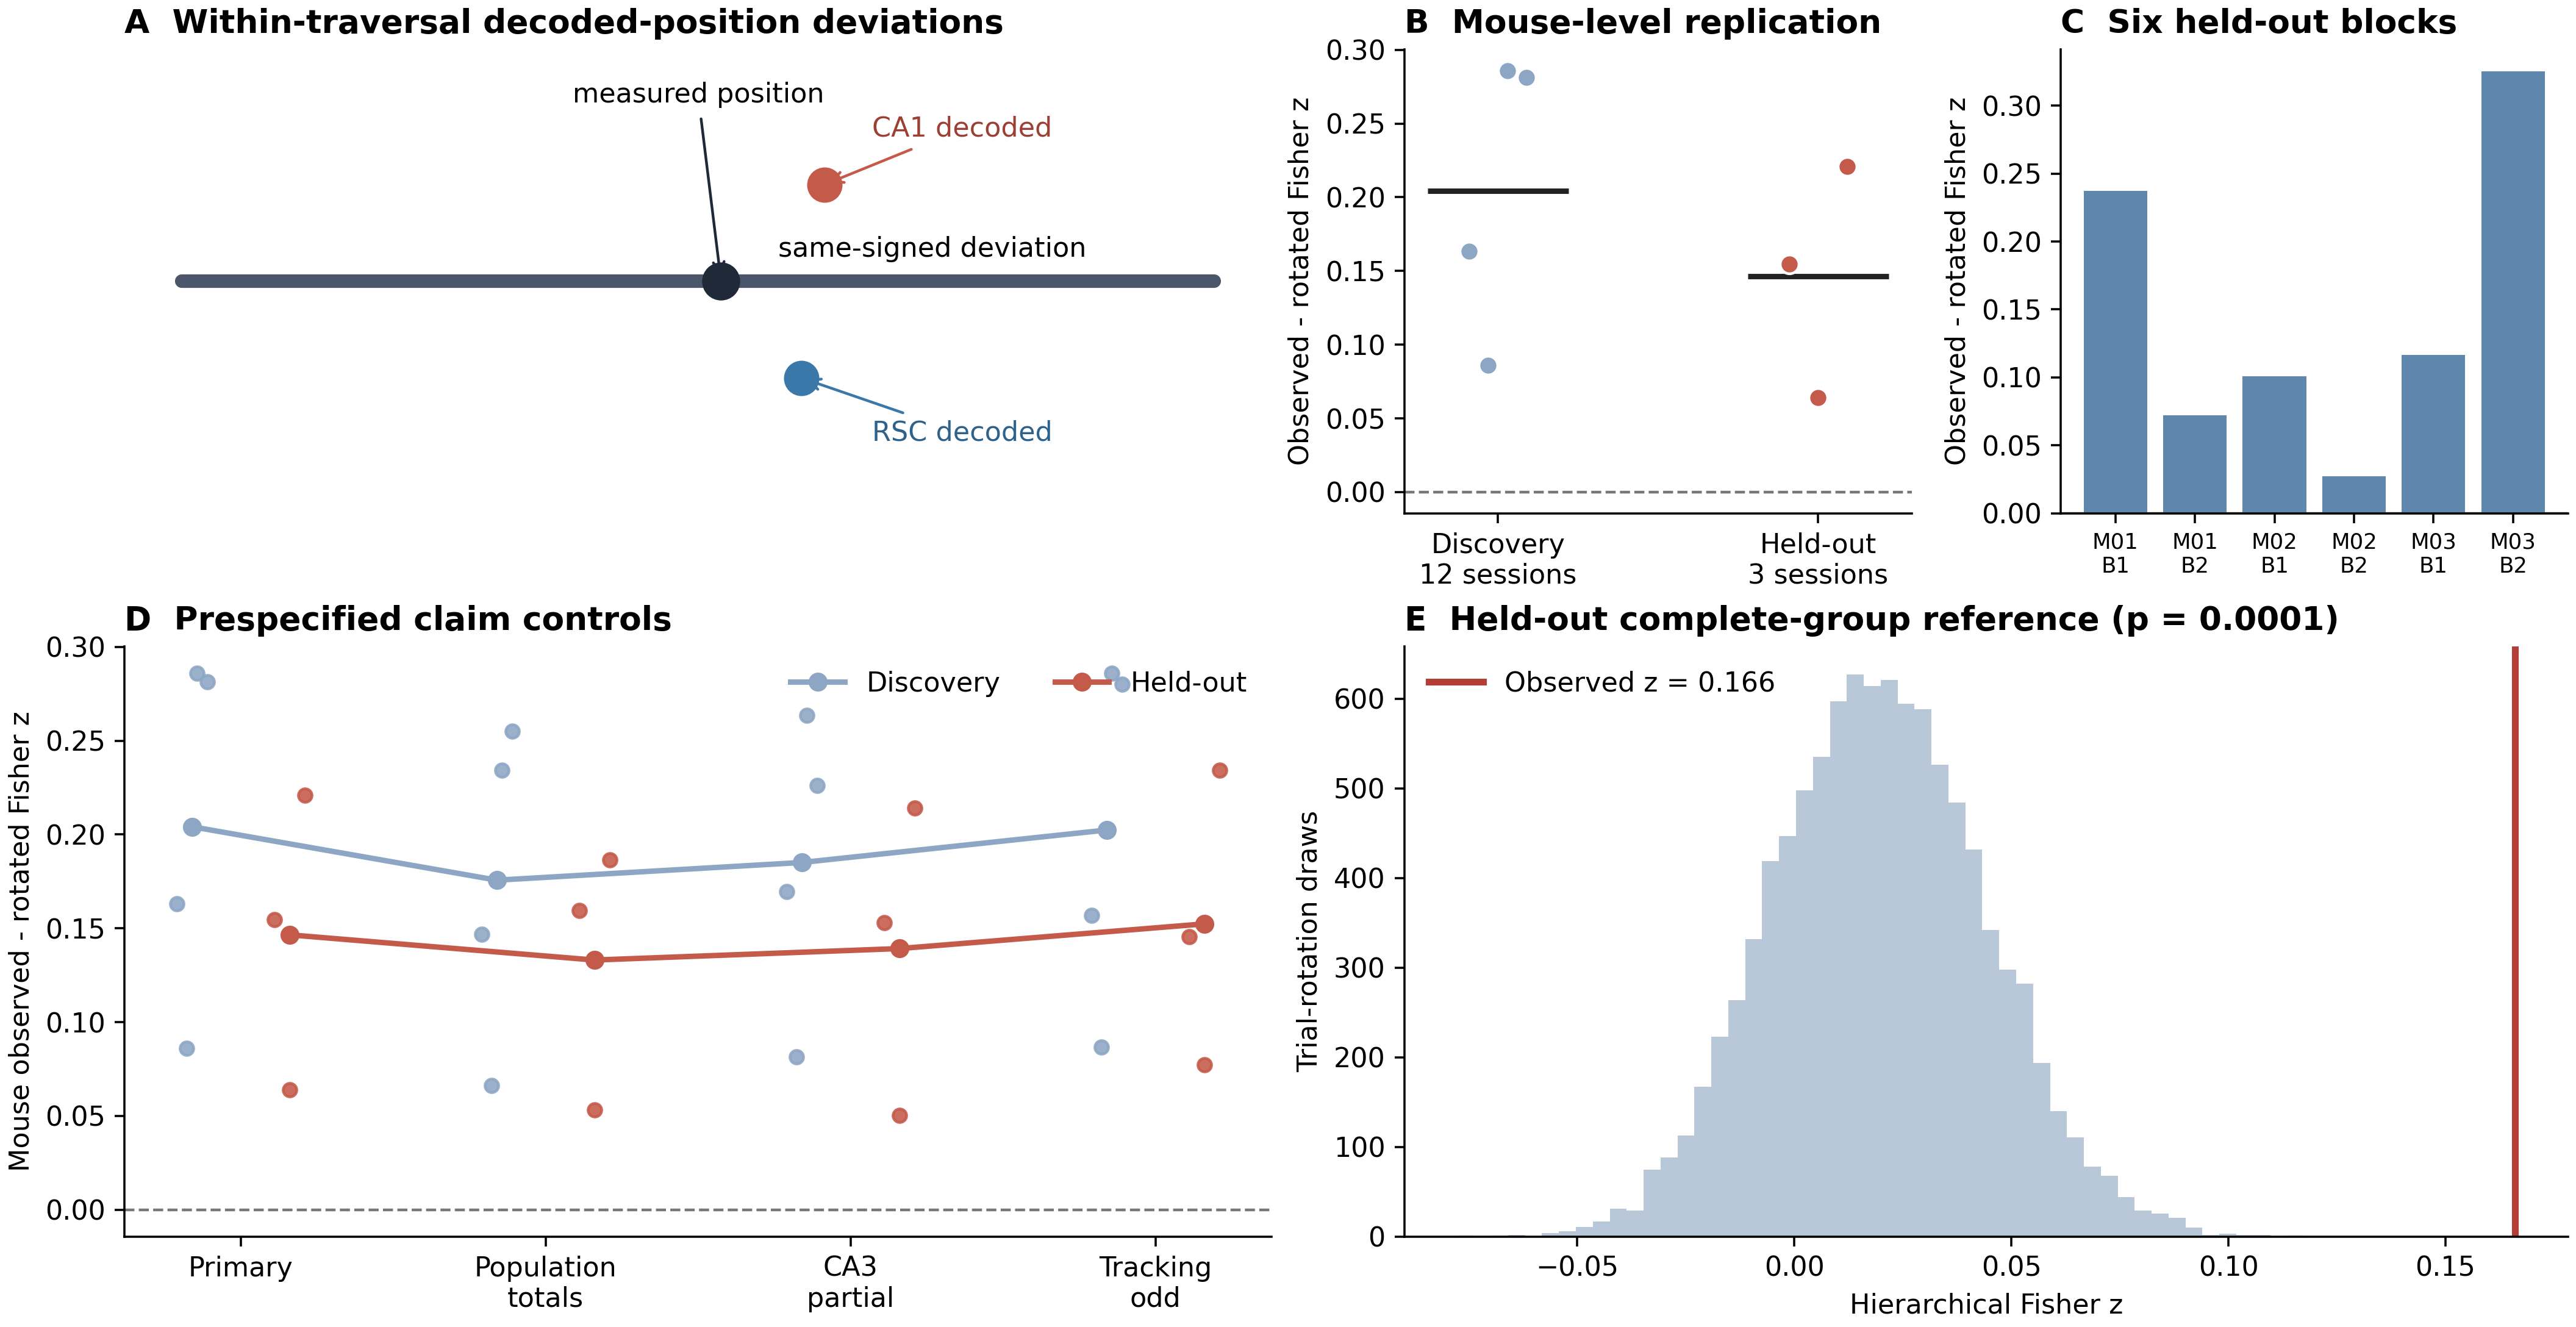
\includegraphics[width=\textwidth]{figure1.png}
\caption{\textbf{CA1 and RSC show coherent held-out position-decoding deviations.} \textbf{A}, Conceptual definition: both independently decoded positions deviate in the same direction from measured position. The analysis correlates covariate-adjusted deviations rather than these raw values. \textbf{B}, Mouse-level observed-minus-rotation Fisher correlations in exploratory and held-out sessions; horizontal bars are cohort means. \textbf{C}, All six held-out maze blocks had positive margins. \textbf{D}, The effect persisted after adjustment for three-area population totals, adjustment for decoded CA3 deviation, and reconstruction from odd tracking frames. Points show mice and lines show equal-mouse means. \textbf{E}, Frozen held-out primary statistic (red) relative to 9,999 complete-product cyclic trial rotations.}
\label{fig:main}
\end{figure*}

\subsection{Population vigor, CA3 deviation, and tracking do not account for the result}

Adding log-transformed CA1, RSC, and CA3 population spike totals to each area's temporal residual model reduced the held-out excess modestly to 0.1331, but the result remained outside all 9,999 rotations ($p=0.0001$; three of three mice positive). Thus the observed sign coordination was not explained solely by population vigor or the simultaneous absence of spikes.

We next removed a cubic function of the independently decoded, aligned CA3 residual from both CA1 and RSC. The held-out excess remained 0.1392 ($p=0.0001$; three of three mice positive). This conditional result does not identify a pathway, but shows that a scalar decoded CA3 displacement did not fully account for the CA1--RSC relation.

A common tracking value can create correlated raw errors when it is subtracted from two decoded estimates. Here, continuous-position and bin-center errors became algebraically identical after projection through the frozen position design; their maximum numerical discrepancy was $3.81\times10^{-12}$. Reconstructing the monotone trajectory from the opposite parity of tracking frames also preserved the held-out excess (0.1524, $p=0.0001$; three of three mice positive). These checks strongly disfavor framewise tracking jitter as the source of the result.

\section{Discussion}

The data support a limited but reproducible phenomenon: within the same traversal and spatial bin, CA1 and deep-layer RSC population decoders tend to deviate in the same direction after measured position, nonlinear speed, and trial order are removed. The relation replicated in sessions that were not used to select the estimator and survived adjustments for population totals and decoded CA3 displacement. This extends coherent spatial-deviation analyses from CA1--visual and CA1--prefrontal systems \citep{saleem2018,tang2019} to the hippocampal--retrosplenial axis.

The result does not imply that CA1 sends an error signal to RSC. Simultaneous deviations could arise from direct or indirect coupling, shared inputs, an unmeasured behavioral variable, or a distributed network state. Only position and speed were available in the released behavior data. Unlike the study of CA1 and visual cortex \citep{saleem2018}, there was no independent licking or choice-error measure with which to identify an animal's subjective position. We therefore use ``decoded-position deviation'' rather than ``subjective position.''

The held-out sessions are a strong safeguard against analysis overfitting but not an independent-animal replication: M01, M02, and M03 were already represented in discovery. Population inference is consequently limited to the four recorded mice. In addition, the source-convention RSC population excluded narrow interneurons but included wide-spiking cells. The literal RSC ``Pyramidal Cell'' sensitivity was not evaluable in all held-out blocks because M01 had four eligible labeled cells per block, below the frozen minimum of five. A new experiment should replicate the result in additional animals with histologically resolved RSC cell classes and behavioral reports of navigation error.

The CA3 conditional analysis offers a concrete next step. Simultaneous decoding from CA3, CA1, and RSC could be extended to lag-resolved or state-space models that ask whether a common positional displacement propagates through the axis, without assuming direction from zero-lag correlation. Such analyses should be preregistered on independent data and should preserve the strict separation between a shared online spatial estimate and a behaviorally validated subjective map.

\section{Methods}

\subsection{Dataset and separation of discovery from confirmation}

We analyzed the navigation recordings released with Gonzalez et al. \citep{gonzalez2026} (DANDI:001695, version 0.260319.2023). Discovery comprised 12 single-maze sessions: M01-20240312/13/14, M02-20240312/13/14, M03-20240621/22/23, and M05-20240729/30/31. Three fixed-condition sessions were sealed for confirmation: M01-20240318, M02-20240318, and M03-20240624. Each confirmation session contained two maze blocks. Before confirmation, code, simulation calibration, input hashes, seed, draw counts, and the complete decision rule were committed publicly. A write-once sentinel was created before the first aligned held-out score.

CA1 and CA3 populations used units labeled ``Pyramidal Cell.'' The primary RSC population followed the source convention \texttt{cell\_type != Narrow Interneuron}. Units required at least 20 locomotor spikes within a block. Blocks required at least ten CA1 and five RSC units and at least 16 accepted traversals per direction.

\subsection{Behavioral coordinate and temporal observations}

Position was linearized by the first principal component and normalized using the first and 99th percentiles within each maze block. Traversals connected the 0.15 and 0.85 endpoints, covered at least 0.70 of the track, and lasted no more than 120 s. Within each traversal, a monotone coordinate was fitted by pool-adjacent-violators regression to even-indexed tracking frames and interpolated to 250-ms nonoverlapping neural windows. Windows required speed above 2.5 cm/s. The decoder used 24 fixed physical bins and was evaluated in central bins 4--19.

\subsection{Conditional-multinomial decoding}

For position bin $x$, area-specific cell probabilities were estimated from training spikes as
\begin{equation}
p_i(x)=\frac{K_i(x)+\alpha}{\sum_j K_j(x)+\alpha N},
\end{equation}
where $K_i(x)$ is the one-bin Gaussian-smoothed spike count for cell $i$, $N$ is the number of included cells, and $\alpha=0.5$. For an observed count vector $\mathbf{k}$ with total $n$, the position likelihood conditioned on $n$ was
\begin{equation}
\log L(x\mid \mathbf{k},n)=\sum_i k_i\log p_i(x)+C(\mathbf{k}),
\end{equation}
with a uniform spatial prior. The decoded position was the posterior mean of the 24 bin centers. When $n=0$, the posterior was uniform and the prediction was 0.5; these windows were retained.

Decoders were fitted separately by area, block, direction, and traversal parity. Even traversals predicted odd traversals and vice versa. No test traversal contributed spikes to its decoder template.

\subsection{Covariate adjustment and record statistic}

At each held-out 250-ms window, signed error was decoded position minus continuous measured coordinate. In each block-by-direction-by-fold record, CA1, RSC, and CA3 errors were separately projected on a fixed design containing 16 true-bin indicators, linear/quadratic/cubic within-bin coordinate, linear/quadratic/cubic standardized speed, and linear/quadratic normalized traversal order. Residuals were averaged within traversal-by-position cells. The primary record statistic was the Pearson correlation of CA1 and RSC residuals, Fisher transformed before hierarchical averaging.

The population-total control added log-transformed CA1, RSC, and CA3 spike totals from each 250-ms window to the residual design. For the CA3 control, a cubic function of the aggregated decoded CA3 residual was removed from both CA1 and RSC before their correlation.

\subsection{Trial-rotation inference}

For every draw and block-by-direction-by-fold stratum, the RSC traversal rows were cyclically shifted by an independently sampled integer from zero through $n-1$. The full RSC row, position columns, and missing-bin mask moved together. The product of these cyclic groups preserves within-traversal spatial structure while breaking same-traversal alignment. All 9,999 draws were aggregated using the same equal fold, direction, block, session-within-mouse, and mouse hierarchy as the observed statistic. One-sided Monte Carlo values used
\begin{equation}
p=\frac{1+\#\{T_{\mathrm{null}}\geq T_{\mathrm{obs}}\}}{1+9999}.
\end{equation}

Before confirmation, 1,000 synthetic null cohorts produced a 5.0\% rejection rate, and 1,000 cohorts with correlation 0.10 produced 99.9\% power using 199-draw calibration tests. The confirmation required positive aggregate excess, $p\leq0.05$, positive margins in all three mice and all leave-one-mouse-out estimates, and positive margins for both directions and both folds.

\section*{Data and code availability}

All analysis code, frozen specifications, calibration draws, discovery outputs, confirmation null banks, provenance manifests, and figures are public at \url{https://github.com/asim-v/ca1-rsc-coherent-position-errors}. Raw data are available from DANDI:001695.

\section*{Acknowledgements}

This study reanalyzes publicly released recordings. We thank the original investigators for making the dataset available.

\begin{thebibliography}{9}
\bibitem[Saleem et al.(2018)]{saleem2018}
Saleem AB, Diamanti EM, Fournier J, Harris KD, Carandini M. Coherent encoding of subjective spatial position in visual cortex and hippocampus. \emph{Nature}. 2018;562:124--127. doi:10.1038/s41586-018-0516-1.

\bibitem[Tang et al.(2019)]{tang2019}
Tang W, Shin JD, Jadhav SP. Coherent coding of spatial position mediated by theta oscillations in the hippocampus and prefrontal cortex. \emph{J Neurosci}. 2019;39:4550--4565. doi:10.1523/JNEUROSCI.2996-18.2019.

\bibitem[Haggerty and Ji(2015)]{haggerty2015}
Haggerty DC, Ji D. Activities of visual cortical and hippocampal neurons co-fluctuate in freely moving rats during spatial behavior. \emph{eLife}. 2015;4:e08902. doi:10.7554/eLife.08902.

\bibitem[Gonzalez et al.(2026)]{gonzalez2026}
Gonzalez J, et al. Subspace communication in the hippocampal-retrosplenial axis. \emph{Nature}. 2026. doi:10.1038/s41586-026-10481-z.

\bibitem[van der Goes et al.(2024)]{vandergoes2024}
van der Goes MS, et al. Coordinated head direction representations in mouse anterodorsal thalamic nucleus and retrosplenial cortex. \emph{eLife}. 2024;13:e82952. doi:10.7554/eLife.82952.
\end{thebibliography}

\end{document}
